\documentclass[a4paper, 11pt]{article}
\usepackage[UTF8]{ctex}
\usepackage{amsmath}
\usepackage{graphicx}
\usepackage{geometry}
\usepackage{listings}
\usepackage{enumerate}
\geometry{scale=0.8}
\usepackage{hyperref}
\linespread{1.5}

\title{
\normalfont \normalsize
\textsc{School of Data and Computer Science, Sun Yat-sen University} \\ [25pt] %textsc small capital letters
\rule{\textwidth}{0.5pt} \\[0.4cm] % Thin top horizontal rule
\huge  T02 CSP and KRR\\ % The assignment title
\rule{\textwidth}{2pt} \\[0.5cm] % Thick bottom horizontal rule
\author{16337110 匡乾, 16337111 赖若潘}
\date{\normalsize\today}
}

\begin{document}
\maketitle
\tableofcontents
\newpage
\section{Q1}
\begin{enumerate}[(a)]
\item
Magic square

	variables:

  $V1,V2,V3,V4,V5,V6,V7,V8,V9$

		\begin{figure}[htbp]
		  \centering
		  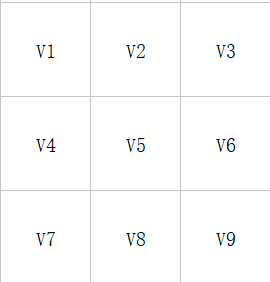
\includegraphics[width=3cm]{1}
		  \caption{变量在图上的分布}
		\end{figure}

	domain:

  $ Dom[Vi]=\{1,2,3, \cdots ,9\} \; (i \in \{1,2,3, \cdots ,9\}) $

	constraints:

		我们很容易可以证明,当每一行,每一列,每一对角线之和相等时,当且仅当它们的和为15。

		证明如下:$(1+2+3+ \cdots +9)/3 = 15$
    \begin{enumerate}[{1.}]
      % all different
      \item C(Vi,Vj):$Vi \ne Vj \; (i,j \in \{1,2,3, \cdots ,9\},i \ne j)$
      % column
      \item C(V1,V4,V7):$V1+V4+V7=15$
      \item C(V2,V5,V8):$V2+V5+V8=15$
      \item C(V3,V6,V9):$V3+V6+V9=15$
      % row
      \item C(V1,V2,V3):$V1+V2+V3=15$
      \item C(V4,V5,V6):$V4+V5+V6=15$
      \item C(V7,V8,V9):$V7+V8+V9=15$
      % diagonal
      \item C(V1,V5,V9):$V1+V5+V9=15$
      \item C(V3,V5,V7):$V3+V5+V7=15$
    \end{enumerate}

\item
Hamiltonian tour

	variables:

		$City_i ( i \in \{1,2, \cdots ,n\} )$ \quad 表示某个城市

		$Road_{(i,j)} ( i,j \in \{1,2, \cdots ,n\},i \ne j )$ \quad 表示某两个城市之间的道路

		$Route_i ( i \in \{1,2, \cdots ,n\} )$ \quad 表示访问的路径

	domain:

		$City_i=\{0,1\}$ \quad 0表示该城市未访问,1表示该城市已访问

		$Road_{(i,j)}=\{0,1\}$ \quad 城市i,城市j之间,无道路用0表示,有道路用1表示

		$Route_i=\{1,2, \cdots ,n\}$ \quad 通过访问城市的顺序来表示访问的路径

	constraints:

		$C(City_1,City_2,\cdots,City_n):\sum_{i=1}^{n}City_i = n$ \quad 保证所有城市都已经访问

		$C(Route_i):Route_i \ne Route_j \; (j \in \{1,\cdots,i\})$ \quad 保证当前访问的城市之前都没有访问过

		$C(Route_i,Route_{i+1}):Road_{(Route_i,Route_{i+1})} = 1 \; (i \in \{1,\cdots,n-1\})$ \quad 保证路径上相邻的两个城市有道路

		$C(Road_{(i,j)},Road_{(j,i)}):Road_{(i,j)}=Road_{(j,i)}$ \quad 保证道路是双向的

\item
Crypto-arithmetic puzzle

	varibles:

		$I,N,T,L,A$

	domain:

		$Dom[I,L,A]=\{1,2,3, \cdots ,9\}$ \quad 首位数字不能为零

		$Dom[N,T]=\{0,1,2,3, \cdots ,9\}$

	constraints:
    \begin{enumerate}[{1.}]
      \item $C(I,N,T,L,A):(I*100+N*10+T)*L=(A*1110+I)$
  		\item $C(I,N):I \ne N$
      \item $C(I,T):I \ne T$
      \item $C(I,L):I \ne L$
      \item $C(I,A):I \ne A$
      \item $C(N,T):N \ne T$
  		\item $C(N,L):N \ne L$
      \item $C(N,A):N \ne A$
      \item $C(T,L):T \ne L$
  		\item $C(T,A):T \ne A$
      \item $C(L,A):L \ne A$
    \end{enumerate}
\end{enumerate}

\section{Q2}
\begin{enumerate}[(a)]
\item
见图(\ref{fig:FC})
\begin{figure}[ht]
  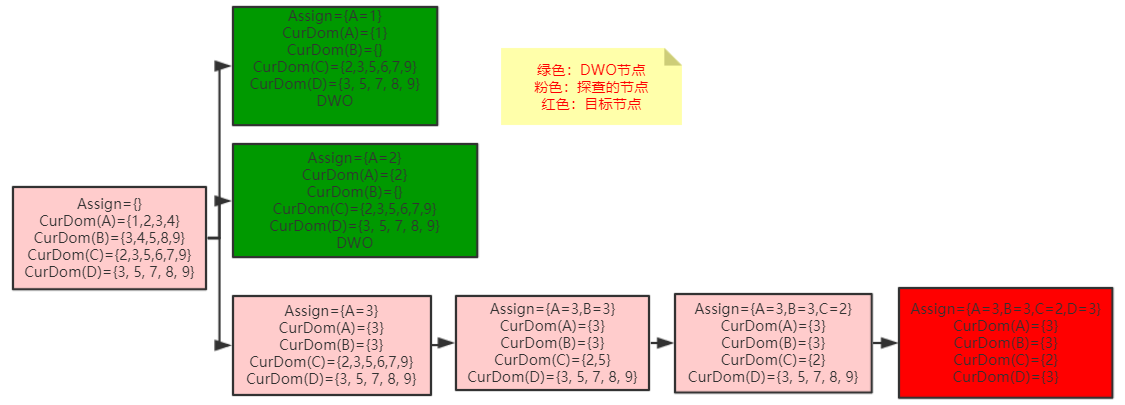
\includegraphics[width=19cm]{2a.PNG}
  \caption{Q2(a): Forward Checking}
  \label{fig:FC}
\end{figure}
\item
\begin{itemize}
  \item 首先进行一次GAC算法,求出变量的值域。
  \begin{itemize}
    \item 对于A=1,B中没有值可以满足约束$A \ge B$,A中删去1。
    \item 对于A=2,B中没有值可以满足约束$A \ge B$,A中删去2。
    \item 对于A=3, 4,B中有B=3可以满足约束$A \ge B$。
    \item 对于B=3, 4,A中有A=4可以满足约束$A \ge B$,C中有C=2满足约束$B>C\ or\ C-B=2$。
    \item 对于B=5, 8, 9,A中没有值可以满足约束$A \ge B$,B中删去5, 8, 9。
    \item 对于C=2, 3, 5, 6,B中有B=9满足$B>C\ or\ C-B=2$,D中都有值满足约束$C \ne D$。
    \item 对于C=7, 9,B中没有值满足$B>C\ or\ C-B=2$,C中删去9。
    \item 对于D中所有值,C中都有值满足约束$C \ne D$。
  \end{itemize}
  所以进行GAC算法后的值域为:
  $D_A$=\{3, 4\},$D_B$=\{3, 4\},$D_C$=\{2, 3, 5, 6\},$D_D$=\{3, 5, 7, 9\}。
  \item 接下来用GAC算法,找到第一个结果,见图(\ref{fig:GAC}):
  \begin{figure}[ht]
    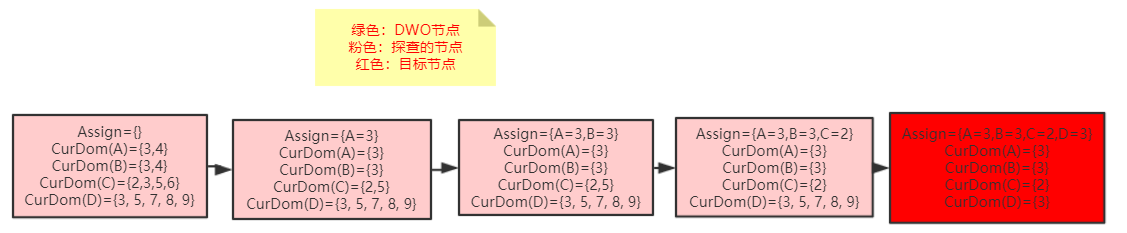
\includegraphics[width=19cm]{2b.PNG}
    \caption{Q2(b): GAC algorithm}
    \label{fig:GAC}
  \end{figure}
\end{itemize}

\end{enumerate}

\section{Q3}
  $S_1:\forall x \forall y(P(x,y) \supset P(y,x)) \iff \forall x \forall y(\lnot P(x,y) \lor P(y,x)) \iff \lnot P(x,y) \lor P(y,x)$

  $S_2:\forall x \forall y \forall z ((P(x,y) \land P(y,z)) \supset P(x,z)) \iff \forall x \forall y \forall z (\lnot(P(x,y) \land P(y,z)) \lor P(x,z)) \iff  \forall x \forall y \forall z (\lnot P(x,y) \lor \lnot P(y,z) \lor P(x,z)) \iff \lnot P(x,y) \lor \lnot P(y,z) \lor P(x,z)$

  $S_3:\forall x \exists y P(x,y) \iff \forall x P(x,f(x)) \iff P(x,f(x))$

  $Enquiry: \forall x P(x,x)$

  refutation:

  \begin{enumerate}[{1.}]
    \item $(\lnot P(x,y),P(y,x))$
    \item $(\lnot P(u,v),\lnot P(v,w),P(u,w))$
    \item $P(z,f(z))$
    \item $\lnot P(a,a)$
    \item R[4,2c]\{u=a, w=a\} $(\lnot P(a,v),\lnot P(v,a))$
    \item R[1,5b]\{y=v, x=a\} $\lnot P(a,v)$
    \item R[3,6]\{z=a,v=f(a)\} ()
  \end{enumerate}

So, we prove that $S_1 \lor S_2 \lor S_3 \supset \forall x P(x,x)$
% 想输入公式吗?
%
% 公式一: $x^2+y^2=z^2$。
%
% 想让公式单列?
% $$x^2+y^2=z^2$$
\section{Q4}
T(X) means that X is the murderer \; (it was thief so I use T to represent the action)

K(X) means that X knows who is the victim

S(X) means that X saw the victim that day

Alexander:

	$\lnot T(A) \to (K(P) \land K(M) \land K(A)) \iff T(A) \lor (\lnot T(P) \land \lnot T(M) \land K(P) \land K(M) \land K(A)) \iff $
	\begin{itemize}
		\item $T(A) \lor K(P) $
		\item $T(A) \lor K(M) $
		\item $T(A) \lor K(A) $
	\end{itemize}

Peter:

	$\lnot T(P) \to (\lnot S(P) \land \lnot K(P)) \iff T(P) \lor (\lnot S(P) \land \lnot K(P)) \iff $
	\begin{itemize}
		\item $T(P) \lor \lnot S(P)$
		\item $T(P) \lor \lnot K(P)$
	\end{itemize}

Michael:

	$\lnot T(M) \to (S(A) \land S(P) \land S(M) \land K(P) \land K(M) \land K(A)) \iff T(M) \lor (S(A) \land S(P) \land S(M) \land K(P) \land K(M) \land K(A)) \iff $
	\begin{itemize}
		\item $T(M) \lor S(A)$
		\item $T(M) \lor S(P)$
		\item $T(M) \lor S(M)$
		\item $T(M) \lor K(P)$
		\item $T(M) \lor K(M)$
		\item $T(M) \lor K(A)$
	\end{itemize}

So now we get the KB as below:
\begin{enumerate}
  \item $(T(A),K(P))$
  \item $(T(A),K(M))$
  \item $(T(A),K(A))$
  \item $(T(P),\lnot S(P))$
  \item $(T(P),\lnot K(P))$
  \item $(T(M),S(A))$
  \item $(T(M),S(P))$
	\item $(T(M),S(M))$
	\item $(T(M),K(P))$
	\item $(T(M),K(M))$
	\item $(T(M),K(A))$
\end{enumerate}

~\\
(a) refutation:
\begin{enumerate}
	\setcounter{enumi}{11}
	\item $ R[4b,7b] \;(T(P),T(M))$
	\item $ R[1b,5b] \;(T(A),T(P))$
\end{enumerate}

Therefore, we can know there is at least one murderer in Peter and Michael while there is at least one murderer in Alexander and Peter. So there is a murderer.Now, we assume that there is only one murderer. And we get $T(A) \oplus T(P) \oplus T(M) 	\Rightarrow $
\begin{enumerate}
	\setcounter{enumi}{13}
	\item $ (\lnot T(A), \lnot T(P)) $
	\item $ (\lnot T(P) , \lnot T(M)) $
	\item $ (\lnot T(M) , \lnot T(A)) $
\end{enumerate}

Query: $ \exists xT(x) $

\begin{enumerate}
	\setcounter{enumi}{16}
	\item $ (\lnot T(x),ans(x)) $
	\item $ R[12,16] \;(T(P),\lnot T(A))$
	\item $ R[13a,18b] \;T(P)$
	\item $ R[17a,19] \{x=P\} \;ans(P)$
\end{enumerate}

In conclusion, Peter is the murderer.

~\\
(b)

By 12 and 13 we actually can't prove that there are only one murderer, there may be two murderers. Prove as below:
\begin{itemize}
	\item When Peter is a murderer, Michael and Alexander can also be the murderer. Then combination of murderers (Peter,Alexander) or (Peter,Michael) are both possible.
	\item When Peter is not a murderer, if and only if Michael and Alexander are both the murderers can ensure the 12 and 13 make sence.
\end{itemize}

Now we asuume that there are two murderers. And we can get $\lnot T(A) \oplus \lnot T(P) \oplus \lnot T(M) 	\Rightarrow $
\begin{enumerate}
	\setcounter{enumi}{20}
	\item $ (T(A), T(P)) $
	\item $ (T(P), T(M)) $
	\item $ (T(M), T(A)) $
\end{enumerate}
Query:$ \exists x \exists y (T(x),T(y)) \ (x \ne y)$
\begin{enumerate}
	\setcounter{enumi}{23}
	\item $ (\lnot T(x), \lnot T(y), ans(x,y)) \ (x \ne y) $
	\item $ R[21,24] \{x=A,y=P\} \;ans(A,P)$
	\item $ R[22,24] \{x=P,y=M\} \;ans(P,M)$
	\item $ R[23,24] \{x=M,y=A\} \;ans(M,A)$
\end{enumerate}

	We get three answers that one suspect is innocent whereas the other two are guilty, and these answers are all possible and correct.

	In conclusion, we can't assume that there was only a single thief.
% 想使条理清晰吗?
%
% \begin{itemize}
% \item 想
% \item 很想
% \item 非常想
% \end{itemize}

%\clearpage
%\bibliography{E:/Papers/LiuLab}
%\bibliographystyle{apalike}
\end{document}


%%% Local Variables:
%%% mode: latex
%%% TeX-master: t
%%% End:
